\documentclass{article}
\usepackage[T1]{fontenc}
\usepackage[preprint]{neurips_2024}
\usepackage{graphicx,booktabs,amsmath,url}
\usepackage[hidelinks]{hyperref}
\title{Chest Radiograph Generation with a VAE}
\author{Pengxuan Zhang\\\small\url{https://github.com/Khal1L1261/chest-xray-vae-homework1}}
\begin{document}
\maketitle
\begin{abstract}
We train a convolutional variational autoencoder (VAE) on chest X-rays. After 40 epochs, held-out torchvision-feature FID is 243.74 and Inception Score is 2.030. Samples capture chest silhouettes but remain blurred and distorted. These results describe a reproducible baseline, not diagnostic validity.
\end{abstract}

\section{Data and model}
We retain the Kaggle dataset's 5,216 training, 16 validation, and 624 test images [1], pooling both diagnostic categories for unconditional generation. Duplicate archive trees are excluded by relative filename. SHA256 checks find no exact file overlap across splits; patient-level independence is not established. Images are converted to grayscale, bilinearly resized to fit $64\times64$ with aspect-ratio-preserving black padding, and scaled to $[0,1]$, without augmentation.

Four stride-2, $4\times4$ encoder convolutions use channels $(32,64,128,256)$ and ReLU. Linear heads map the flattened $256\times4\times4$ tensor to 64-dimensional $\mu$ and $\log\sigma^2$. Reparameterization samples $z=\mu+\sigma\odot\epsilon$, $\epsilon\sim\mathcal N(0,I)$ [2]. A linear projection and four transposed convolutions reverse the encoder. Sigmoid outputs parameterize a Bernoulli surrogate for grayscale pixels. There are 2,168,641 parameters.

\section{Training protocol and learning curves}
We minimize a one-sample estimate of the negative evidence lower bound:
\begin{equation}
\mathcal L=\operatorname{BCE}_{\rm sum}(x,\hat x)
+\tfrac12\sum_{j=1}^{64}(\mu_j^2+\exp(\ell_j)-1-\ell_j),\quad \ell=\log\sigma^2.
\end{equation}
Terms are summed within each image, then averaged over the batch ($\beta=1$); log-variance is clamped to $[-20,20]$. Adam uses learning rate $2\times10^{-4}$, batch size 64, 40 epochs, gradient clipping at 10, seed 42, and no schedule. PyTorch 2.10.0+cu126 runs on an RTX 3060 Laptop GPU (6 GB). Epoch loops total 57.5 seconds, excluding setup, checkpoint writes, and evaluation. Lowest validation loss selects epoch 40; validation sampling has a fixed seed.

\begin{figure}[!htbp]
\centering
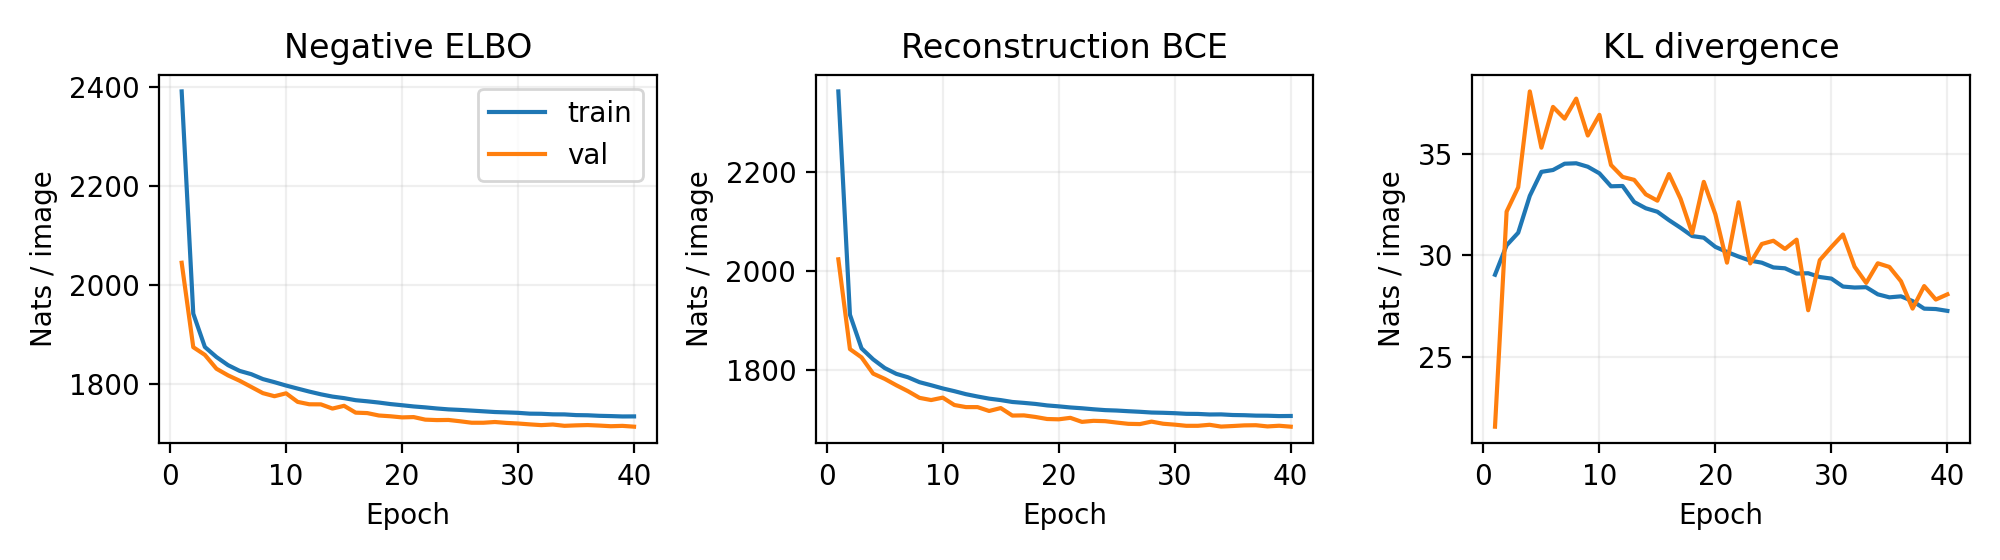
\includegraphics[width=\linewidth]{../results/loss_curves.png}
\caption{Recorded losses (nats/image): training averages during updates and validation after each epoch. BCE decreases; KL stays nonzero.}
\end{figure}

\section{Held-out evaluation and generated examples}
Following the Ignite tutorial [3], we generate 624 prior samples (seed 31415) and compare them with all 624 test images. Both sets are repeated into RGB, bilinearly resized to $299\times299$ with antialiasing, and ImageNet-normalized. Torchvision Inception-v3 ImageNet weights supply 2,048-dimensional pooled features to Ignite FID and 1,000-class softmax probabilities to Ignite IS; the internal input transform is disabled. This explicit protocol differs from clean-fid and the tutorial's default feature configuration.

\begin{table}[!htbp]
\centering
\caption{Measured results; losses are nats/image. IS split SD is across ten disjoint, nearly equal groups, not a confidence interval.}
\begin{tabular}{lr@{\qquad}lr}
\toprule
Quantity & Value & Quantity & Value \\
\midrule
Initial train loss & 2391.80 & Final train loss & 1733.93 \\
Best validation loss & 1713.11 & Test loss & 1694.00 \\
Test BCE & 1667.75 & Test KL & 26.25 \\
FID ($\downarrow$) & 243.74 & Full-set IS ($\uparrow$) & 2.030 \\
\multicolumn{3}{l}{Ten-split IS (mean $\pm$ SD)} & $1.982\pm0.081$ \\
\bottomrule
\end{tabular}
\end{table}

\begin{figure}[!htbp]
\centering
\begin{minipage}[c]{0.30\linewidth}
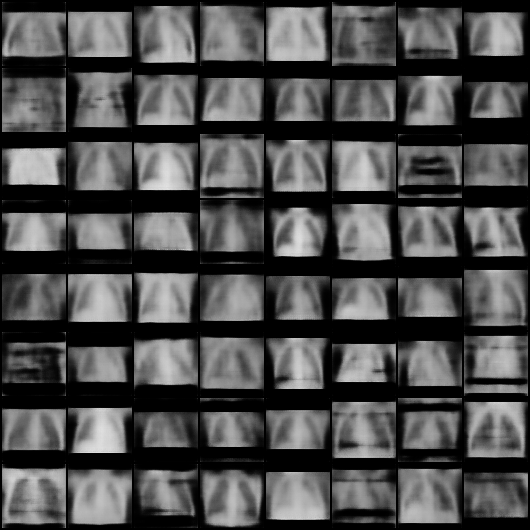
\includegraphics[width=\linewidth]{../results/generated.png}
\end{minipage}\hfill
\begin{minipage}[c]{0.59\linewidth}
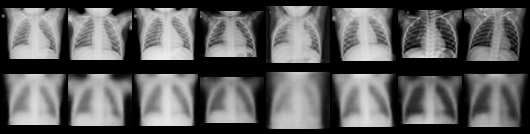
\includegraphics[width=\linewidth]{../results/reconstructions.png}
\small Top: eight validation images. Bottom: deterministic reconstructions obtained by decoding posterior means.
\end{minipage}
\caption{Left: all 64 prior samples (seed 123), without quality-based selection. Black borders originate from preprocessing. Figure and metric seeds differ.}
\end{figure}

\section{Discussion and limitations}
Loss decreases rapidly, then more slowly. Nonzero KL means the posterior is not identically the prior, but does not prove all latent dimensions are active. Samples vary in brightness and shape; fine structures are blurred and some silhouettes malformed. Reconstructions condition on real images, whereas prior samples test unconditional generation. Low resolution, pixelwise reconstruction, and imperfect prior matching may contribute to these limitations; no ablation isolates their effects.

Only one training seed is tested. The tiny validation set makes checkpoint selection uncertain; 624-image FID has finite-sample limitations. ImageNet categories do not represent medical findings, so neither metric establishes anatomical correctness.

\small
\noindent\textbf{References}\par
\noindent [1] P. Mooney. Chest X-Ray Images (Pneumonia). Kaggle. \url{https://www.kaggle.com/datasets/paultimothymooney/chest-xray-pneumonia}.\par
\noindent [2] D. P. Kingma and M. Welling. Auto-Encoding Variational Bayes. ICLR, 2014.\par
\noindent [3] PyTorch-Ignite. GAN evaluation using FID and IS. \url{https://pytorch-ignite.ai/blog/gan-evaluation-with-fid-and-is/}.
\end{document}
